\documentclass[12pt,a4paper]{report}

% --- PACOTES BÁSICOS E CORES ------------
\usepackage[utf8]{inputenc}
\usepackage[brazil]{babel}

% Definido uma única vez com as margens ABNT corretas
\usepackage[top=3cm, left=3cm, right=2cm, bottom=2cm, headsep=1.2cm]{geometry} 
\usepackage{indentfirst} 
\usepackage{setspace}     
\onehalfspacing          
\usepackage{mathptmx}
\usepackage{amsmath}
\usepackage{amssymb}
\usepackage{etoolbox}    
\usepackage{titlesec}    
\usepackage{graphicx}
\usepackage{float}
\usepackage[table]{xcolor} % Declarado apenas uma vez aqui
\usepackage{array}
\usepackage{caption}
\setlength{\belowcaptionskip}{20pt}

% --- CONFIGURAÇÃO DE CABEÇALHO E NUMERAÇÃO -------------------------------------
\usepackage{fancyhdr}
\setlength{\headheight}{14.5pt}
\pagestyle{fancy}
\fancyhf{} 
\fancyhead[R]{\thepage} 
\renewcommand{\headrulewidth}{0pt} 

% Garante que inícios de capítulo normais usem o estilo fancy (número no topo)
\patchcmd{\chapter}{\thispagestyle{plain}}{\thispagestyle{fancy}}{}{}

% --- FORMATAÇÃO DE TÍTULOS (Capítulos e Seções) ---
\titleformat{\chapter}[hang]
{\normalfont\bfseries\normalsize}{\thechapter}{0.5em}{\MakeUppercase}
\titlespacing*{\chapter}{0pt}{0pt}{1.5em}

% Seção
\titleformat{\section}
{\normalfont\normalsize}{\thesection}{0.5em}{\MakeUppercase}
\titlespacing*{\section}{0pt}{1.5em}{1em}

% Subseção
\titleformat{\subsection}
{\normalfont\bfseries\normalsize}{\thesubsection}{0.5em}{}
\titlespacing*{\subsection}{0pt}{1.5em}{1em}

% --- Configurações de parágrafo ---
\setlength{\parindent}{1.25cm} 
\setlength{\parskip}{0pt}      
\usepackage[titles]{tocloft}

% Configuração da Bibliografia
\usepackage{csquotes}
\usepackage[style=abnt, backend=biber]{biblatex} 
\addbibresource{referencias.bib}

\usepackage{ragged2e} 

% Para Fluxograma (Removidas as duplicatas de pacotes)
\usepackage{tikz}
\usetikzlibrary{shapes.geometric, arrows.meta, positioning, calc, shapes.symbols}
\definecolor{mygreen}{HTML}{C5F2C7}
\usepackage{fontawesome5}
\usepackage{enumitem}

% --- INÍCIO DO DOCUMENTO -------------------------------------------
\begin{document}

% 1. CAPA (Não conta, não numera)
\pagestyle{empty}
\begin{center}
    \thispagestyle{empty}

    \begin{figure}[h]
    \centering
    
\includegraphics[width=0.5\textwidth]{imagens/logo.jpg}
    \label{fig:logo}
\end{figure} 

    \textbf{UNIVERSIDADE FEDERAL DO VALE DO SÃO FRANCISCO} \\
    \textbf{ CURSO DE GRADUAÇÃO EM ENGENHARIA DA COMPUTAÇÃO} \\[4cm]
    
    \textbf{SEU NOME AQUI} \\[5cm]
    
    \textbf{\Large Arquivo Latex - Desenvolvido por Julia Cardoso Reis} 

    \vfill % Esta "mola" empurra o texto abaixo para o final da página
    
    JUAZEIRO - BA \\ 
    2026             
\end{center}
\clearpage

% --- INÍCIO DA CONTAGEM (Folha de Rosto = Página 1) ---------------------------------
\pagenumbering{arabic} 
\pagestyle{empty} % Conta ocultamente

% Folha de Rosto
\begin{center}
    \thispagestyle{empty}
    
    \textbf{UNIVERSIDADE FEDERAL DO VALE DO SÃO FRANCISCO} \\
    \textbf{CURSO DE GRADUAÇÃO EM ENGENHARIA DE COMPUTAÇÃO} \\[4cm]
    
    \textbf{SEU NOME AQUI} \\[5cm]
    
    \textbf{\Large Arquivo Latex - Desenvolvido por Julia Cardoso Reis} \\ [3cm]

    % --- BLOCO DE TEXTO À DIREITA ---
    \hspace{0.45\textwidth} % Empurra a caixa para a direita
    \begin{minipage}{0.5\textwidth} % Cria a caixa com 50% da largura da folha
        \small % Fonte um pouco menor, como é comum na folha de rosto
        \begin{singlespace} % Espaçamento simples apenas neste bloco
            Trabalho de Conclusão de Curso apresentado como requisito parcial para obtenção do título de Bacharel em Engenharia de Computação, pela Universidade Federal do Vale do São Francisco. 
            
            \vspace{1cm}
            Orientador: Prof. Dr. Jairson Barbosa Rodrigues
        \end{singlespace}
    \end{minipage}

    \vfill 
    
    JUAZEIRO - BA \\ % Removido o \textbf daqui
    2026             % Removido o \textbf daqu
\end{center}
\clearpage

% Folha de Aprovação
\begin{center}
    \thispagestyle{empty}
    
    \textbf{UNIVERSIDADE FEDERAL DO VALE DO SÃO FRANCISCO} \\
    \textbf{CURSO DE GRADUAÇÃO EM ENGENHARIA DE COMPUTAÇÃO} \\[1.5cm]
    
    \textbf{FOLHA DE APROVAÇÃO} \\[1.5cm]
    
    \textbf{SEU NOME AQUI} \\[1.5cm]
    
    \textbf{\Large Arquivo Latex - Desenvolvido por Julia Cardoso Reis} \\[1.5cm]

    % --- BLOCO DE NOTA DE APRESENTAÇÃO ---
    \hspace{0.45\textwidth}
    \begin{minipage}{0.5\textwidth}
        \small
        \begin{singlespace}
            Trabalho de Conclusão de Curso apresentado como requisito parcial para obtenção do título de Bacharel em Engenharia de Computação, pela Universidade Federal do Vale do São Francisco.
        \end{singlespace}
    \end{minipage} \\[1.5cm]

    \textbf{Aprovado em: XX de -MÊS- de 202X} \\[1.5cm]

    \textbf{Banca Examinadora} \\[1.2cm]

    % --- ASSINATURAS ---
     \rule{10cm}{0.1mm} \\
    \textbf{Avaliador 1 da banca, Dr. } \\
    \textbf{CECOMP / UNIVASF} \\[1.1cm]

    \rule{10cm}{0.1mm} \\
    \textbf{Avaliador 2 da banca, MSc.} \\
    \textbf{CECOMP / UNIVASF} \\[1.1cm]

     \rule{10cm}{0.1mm} \\
    \textbf{Jairson Barbosa Rodrigues, Dr.} \\
    \textbf{CECOMP / UNIVASF}
    
\end{center}
\clearpage

% --- ELEMENTOS PRÉ-TEXTUAIS (Centralizados) --------------------------
\titleformat{\chapter}[block]{\normalfont\bfseries\normalsize\filcenter}{}{0pt}{\MakeUppercase}

\thispagestyle{empty}

\vspace*{\fill}

\begin{flushright}
    \begin{minipage}{0.6\textwidth} % A caixa de texto da epígrafe costuma ser um pouco maior
        \textit{"Se vi mais longe foi por estar de pé sobre ombros de gigantes"} \\
        (TROYAN, 2004)
    \end{minipage}
\end{flushright}

\vspace{2cm}
\clearpage

\begin{center}
    \textbf{\normalsize AGRADECIMENTOS}
\end{center}

\vspace{1cm}

Gostaria de dedicar este trabalho à todos que me acompanharam nesta jornada especialmente 


\thispagestyle{empty}
\clearpage

\input{resumo}
\clearpage

\begin{center}
    \textbf{\normalsize ABSTRACT}
\end{center}

\vspace{1cm}

\noindent % Garante que comece na margem esquerda
\begin{justify} % Força o alinhamento justificado sem interferências
Lorem ipsum dolor sit amet, consectetur adipiscing elit. Sed non risus. Suspendisse lectus tortor, dignissim sit amet, adipiscing nec, ultricies sed, dolor. Cras elementum ultrices diam, at varius nisl fermentum in. Maecenas ligula massa, varius a, semper congue, euismod non, mi. Proin porttitor, orci nec nonummy molestie, enim est eleifend mi, non fermentum diam nisl sit amet erat. Duis semper, purus vitae facilisis gravida, nulla lorem tincidunt elit, ut pretium sapien sapien nec justo. Duis arcu massa, scelerisque vitae, consequat in, pretium a, enim. Pellentesque congue, augue id cursus tempor, sapien justo aliquet urna, ut blandit turpis nulla vel quam. Ut in risus volutpat libero pharetra tempor, in facilisis elit luctus. Curabitur sit amet mauris eget lorem varius tincidunt.
\end{justify}

\vspace{1.5cm}

\noindent \textbf{Keywords:}Lorem; ipsum; dolor sit amet; consectetur adipiscing elit.

\thispagestyle{empty}
\clearpage

\input{pretextual/ilustracoes}
\clearpage

% tabelas.tex
\listoftables
\thispagestyle{empty} % Garante que não apareça número nesta página
\clearpage

\begin{center}
    \textbf{\normalsize LISTA DE ABREVIATURAS E SIGLAS}
\end{center}

\vspace{1cm}

% --- Aumenta o espaçamento vertical entre as linhas da tabela ---
\renewcommand{\arraystretch}{1.8}

\begin{tabular}{p{2cm} l}
    AP  & Aprendizado de Máquina \\
    PKC  & \textit{Public Key Criptography} \\
  
    
\end{tabular}

\thispagestyle{empty}
\clearpage

\tableofcontents
\clearpage

% --- INÍCIO DA PARTE TEXTUAL (Mostrar numeração no topo direito) ----------------------
\pagestyle{fancy} 
\titleformat{\chapter}[hang]{\normalfont\bfseries\normalsize}{\thechapter}{0.5em}{\MakeUppercase}

\chapter{INTRODUÇÃO}

Lorem ipsum dolor sit amet, consectetur adipiscing elit. Sed non risus. Suspendisse lectus tortor, dignissim sit amet, adipiscing nec, ultricies sed, dolor. Cras elementum ultrices diam, at varius nisl fermentum in. Maecenas ligula massa, varius a, semper congue, euismod non, mi. Proin porttitor, orci nec nonummy molestie, enim est eleifend mi, non fermentum diam nisl sit amet erat.


\section{JUSTIFICATIVA}

Lorem ipsum dolor sit amet, consectetur adipiscing elit. Sed non risus. Suspendisse lectus tortor, dignissim sit amet, adipiscing nec, ultricies sed, dolor. Cras elementum ultrices diam, at varius nisl fermentum in. Maecenas ligula massa, varius a, semper congue, euismod non, mi. Proin porttitor, orci nec nonummy molestie, enim est eleifend mi, non fermentum diam nisl sit amet erat. 



\section{OBJETIVO GERAL}

Sair da UNIVASF e nunca mais pisar lá.

\section{OBJETIVOS ESPECÍFICOS}

\begin{itemize}
    \item Formar;
    \item Fazer mestrado;
    \item Ir pra iniciativa privada;
    \item Concurso público;
    \item Iniciar terapia; 
\end{itemize}

\section{ORGANIZAÇÃO DO TRABALHO}

Este trabalho está estruturado do jeito para.......
\chapter{TRABALHOS RELACIONADOS}

Neste capítulo serão abordados os trabalhos que contribuem para o momento presente desta área de pesquisa.




\chapter{REFERENCIAL TEÓRICO}

Nesta seção, será descrita a base teórica da pesquisa aqui desenvolvida.


\section{INTELIGÊNCIA ARTIFICIAL}

A inteligência artificial é o estudo de agentes que recebem percepções do ambiente e realizam ações. Um agente opera autonomamente, percebe seu ambiente e persiste por um longo período de tempo, adaptando-se a mudanças e perseguindo seu objetivo \cite{russell2003ai}.

\begin{figure}[H]
    \centering
    \caption{Campos de estudo de Inteligência Artifial.}
    \label{fig:conjunto-ia}
    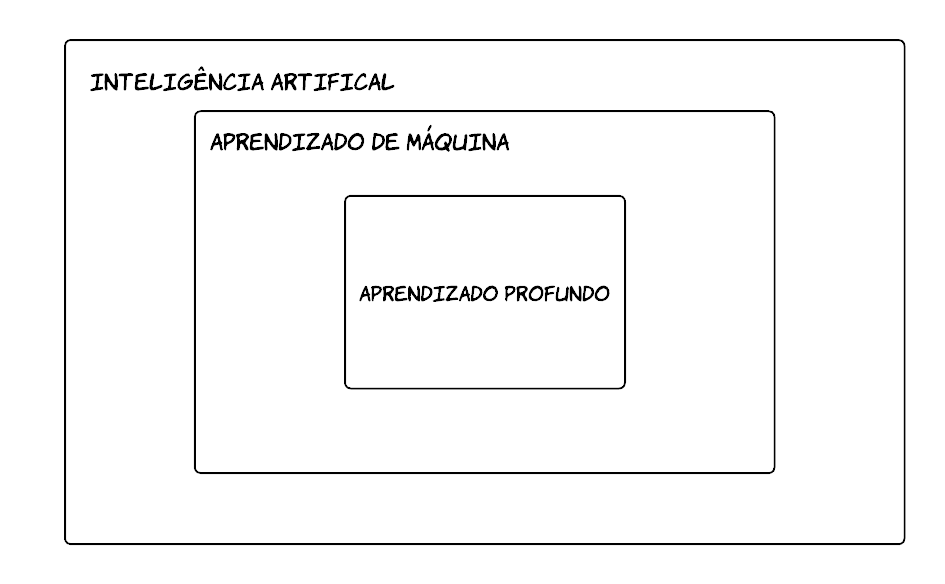
\includegraphics[width=0.9\textwidth]{imagens/conjunto-ia-ml-dl-PTBR.png}


    
    {\footnotesize \textbf{Fonte:} A Autora (2026).}
\end{figure}


\subsection{Aprendizado de Máquina}

 O ciclo descrito é mostrado na figura abaixo:

\begin{figure}[htbp]
    \centering
    \caption{Fluxograma da construção de um algoritmo de aprendizado de máquina.}
    \label{fluxograma-ai-ml}

    % 1. Definimos a caixa de ícone FORA do tikzpicture
    \newcommand{\iconbox}[1]{%
        \tikz[baseline=-0.5ex]{%
            \node[fill=white, text=black, rounded corners=2pt, inner sep=4pt, minimum height=0pt, minimum width=0pt, text width=]{\Large #1};%
        }\\[0.2cm]%
    }

    % 2. AJUSTE AQUI: Mudamos de \textwidth para 0.8\textwidth (80% do tamanho da linha)
    \resizebox{0.7\textwidth}{!}{%
    \begin{tikzpicture}[
        % Espaçamento global entre os nós
        node distance=1.5cm and 1cm,
        % Estilo base para todos os nós
        base/.style={
            fill=white,         % Alterado de 'mygreen' para branco
            draw=black,         % Mantém a borda preta
            text=black,         % Garante o texto em preto
            font=\sffamily\bfseries\small, 
            text width=4.2cm, 
            align=center, 
            minimum height=2.8cm, 
            inner sep=0.3cm
        },
        % Estilo para as caixas retangulares
        box/.style={
            base,
            rectangle, 
            rounded corners=4pt
        },
        % Estilo para a caixa inicial (formato de pílula)
        oval/.style={
            base,
            rectangle,
            rounded corners=1.4cm
        },
        % Estilo das setas
        arrow/.style={
            ->, 
            =latex, 
            draw=black!70,
            thick
        }
    ]

    % ==================== NÓS DO FLUXOGRAMA ====================
    \node (n1) [oval] {\iconbox{\faDatabase}1 - COLETA DE DADOS\\(DADOS BRUTOS)};

    \node (n2) [box, right=of n1] {\iconbox{\faCogs}2 - PROCESSAMENTO PARA NORMALIZAÇÃO E PADRONIZAÇÃO DOS DADOS};

    \node (n3) [box, right=of n2] {\iconbox{\faRobot}3 - TREINAMENTO DO MODELO};

    % Posicionando a segunda linha de nós
    \node (n4) [box, below=2cm of n3] {\iconbox{\faChartLine}4 - APLICAÇÃO EM CENÁRIO REAL};

    \node (n5) [box, left=of n4] {\iconbox{\faBrain}5 - TOMADA DE DECISÃO INTELIGENTE PELO ALGORITMO DE ML};

    % ==================== SETAS DE CONEXÃO ====================
    \draw [arrow] (n1) -- (n2);
    \draw [arrow] (n2) -- (n3);

    % Seta do N3 para o N4 
    \draw [arrow] (n3.south) -- ++(0,-0.8) -| ([xshift=0.8cm]n4.east) -- (n4.east);

    % Seta do N4 para o N5
    \draw [arrow] (n4) -- (n5);

    \end{tikzpicture}%
    }

    \vspace{0.4cm}
    {\footnotesize \textbf{Fonte:} Feitosa; Santos; Sousa (2023).}
\end{figure}

\vspace{2.0cm}




\section{CRIPTOGRAFIA}

Para entender o que é a criptografia, é necessário antes inteirar-se de alguns conceitos-base. Texto claro é a mensagem original, legível. Texto cifrado é quando a mensagem original é codificada. O processo de transformar um texto claro em um texto cifrado é chamado de \textbf{cifração}; converter um texto cifrado em um texto claro novamente é denominado \textbf{decifração}.

\begin{table}[H]
    \centering
    \caption{Conceitos base da criptografia.}
    \label{conceitos_cripto}

    \begin{tabular}{|p{4cm}|p{10cm}|}
        \hline
        \rowcolor[HTML]{EFEFEF} 
        \multicolumn{1}{|c|}{\textbf{Conceito Base}} & \multicolumn{1}{c|}{\textbf{Definição}} \\ \hline
        Texto Claro & Mensagem que deve ser protegida, denominada \textit{M}. \\ \hline
        Texto Cifrado & Mensagem cifrada, denominada \textit{C}. \\ \hline
        Chave & Valor numérico utilizado por um algoritmo para cifrar uma mensagem, fazendo com que a mensagem original seja recuperável mediante utilização deste valor. \\ \hline
        Cifração & Método utilizado para transformar uma mensagem \textit{M}. Sendo \textit{E} uma função de cifração e \textit{k} uma chave, então cifrar pode ser definido como $E_k(M) = C$. \\ \hline
        Decifração & Método para recuperar a mensagem original. Sendo \textit{D} uma função de decifração e \textit{k} uma chave, então decifrar pode ser definido como $D_k(C) = M$. \\ \hline
    \end{tabular}

    \vspace{0.4cm}
    {\footnotesize \textbf{Fonte:} A Autora (2026).}
\end{table}




\subsection{A Criptogrfia Simétrica - Chave Secreta Compartilhada}


A PKC depende das chamadas \textit{trapdoor functions}: são funções matemáticas que são simples de se calcular, ao passo que,  suas funções matemáticas inversa possuem um grau de complexidade matemática . Para explicar tal lógica vamos utilizar como exemplo a potenciação abaixo:

\begin{equation}
   3^6 = 759 
  \label{eq:cifra_publica_funcao}
\end{equation}











\chapter{METODOLOGIA}

Metodologia e os materiais serão descritos neste capítulo


\section{LEGENDA}


\begin{description}[leftmargin=*, widest=FP]
    \item[\textbf{TP} (True Positive):] Verdadeiro Positivo. Representa o número de instâncias em que o modelo previu corretamente a classe positiva.
    \item[\textbf{TN} (True Negative):] Verdadeiro Negativo. Indica a quantidade de instâncias em que o modelo previu corretamente a classe negativa.
\end{description} 



\section{CRONOGRAMA DE ATIVIDADES}

\begin{figure}[htbp]
    \centering
    \caption{Cronograma de atividades do semestre (Agosto -- Dezembro).}
    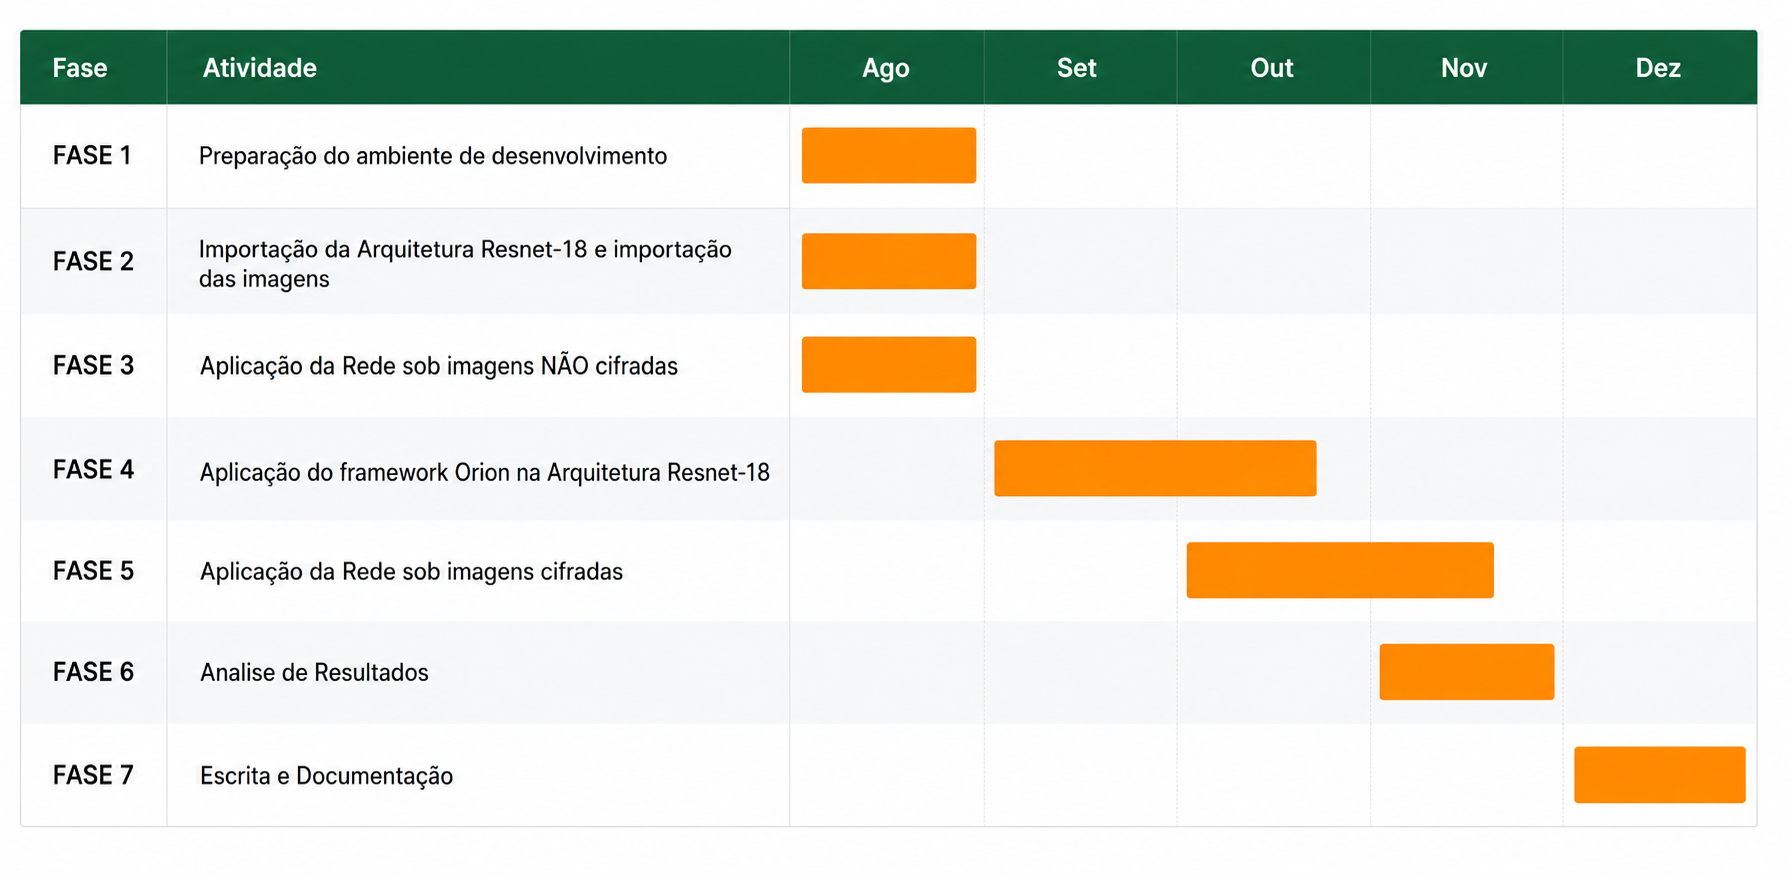
\includegraphics[width=1.0\textwidth]{imagens/cronograma-atv.png}
    \label{fig:cronograma-agosto-dezembro}
    
\end{figure}
\chapter{CONCLUSÃO}

Esse estudo investigativo buscou avaliar o desempenho de modelos de Aprendizagem de Máquina para....(continua)

% --- REFERÊNCIAS ---
\titleformat{\chapter}[block]{\normalfont\bfseries\normalsize\filcenter}{}{0pt}{\MakeUppercase}
\titlespacing*{\chapter}{0pt}{0pt}{1.5em}

\RaggedRight 
\printbibliography[title={REFERÊNCIAS}]

\end{document}